\subsection{Heading autopilot}\label{sec:prob1.1}
\subsubsection*{Analysis of ship characteristics}
To be able to model the ship in a good way we ran many simulations with different rudder angle and measured the steady-state yaw rate. We then made a $\delta-r$ plot of the result. Since the ship was turning port while giving a positive rudder command, this plot the rest of the assignment is made with a fixed gain of -1 on $\delta_c$.

\begin{figure}[H]
    \centering
    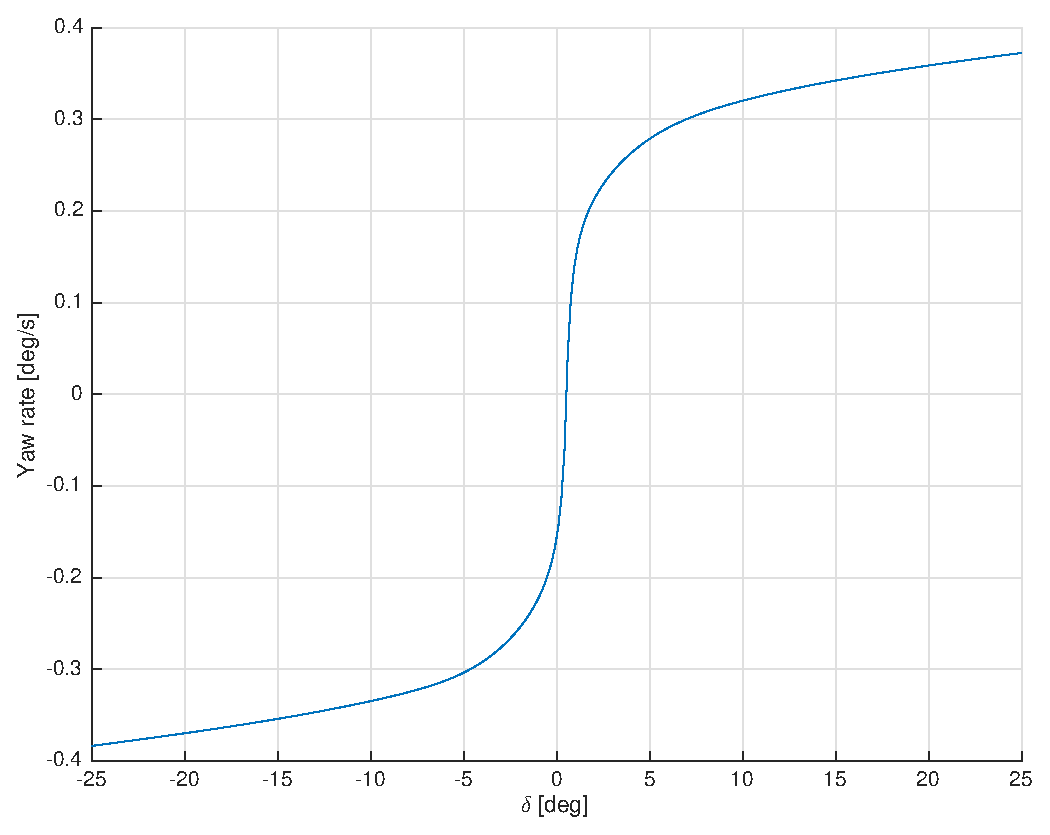
\includegraphics[width=0.9 \textwidth]{task1.4/Task1_4_delta_r_plot}
    \caption{$\delta - r$ plot}
    \label{fig:delta-r-plot}
\end{figure}

From figure \ref{fig:delta-r-plot} we clearly see the non-linear behavior of the ship. This motivates a 1-DOF heading model i.e. first- or second order Monoto model with non-linear extensions. To further investigate the effect of the non-linear characteristics of this ship, we compare the actual response with different models at different rudder angles. It should also be noticed that the ship has a constant drift to starboard with $\delta_c=0$, as seen by the curve not passing through the origin. We compensate for this through the rest of the modeling part by adding a fixed rudder angle of $0.52\degree$ to the rudder input. We only need this correction while estimating the model parameters. In a closed loop, the integral effect will cancel both this drift and drift caused by wind, current and waves.

\subsubsection*{2. order linear Nomoto}

\begin{equation}
\begin{split}
	\frac{r}{\delta}(s) = \frac{K_\nu (1+T_3 s)}{(1+T_1 s) (1+T_2 s) } \\
	T_1 T_2 \dddot{\psi} + (T_1+T_2)\ddot{\psi} +\dot{\psi} = K(\delta+T_3 \dot{\delta})
\end{split}
\end{equation}

The second order Nomoto model follows the ship´s overshoot some, but not enough.

\begin{figure}[H]
    \centering
    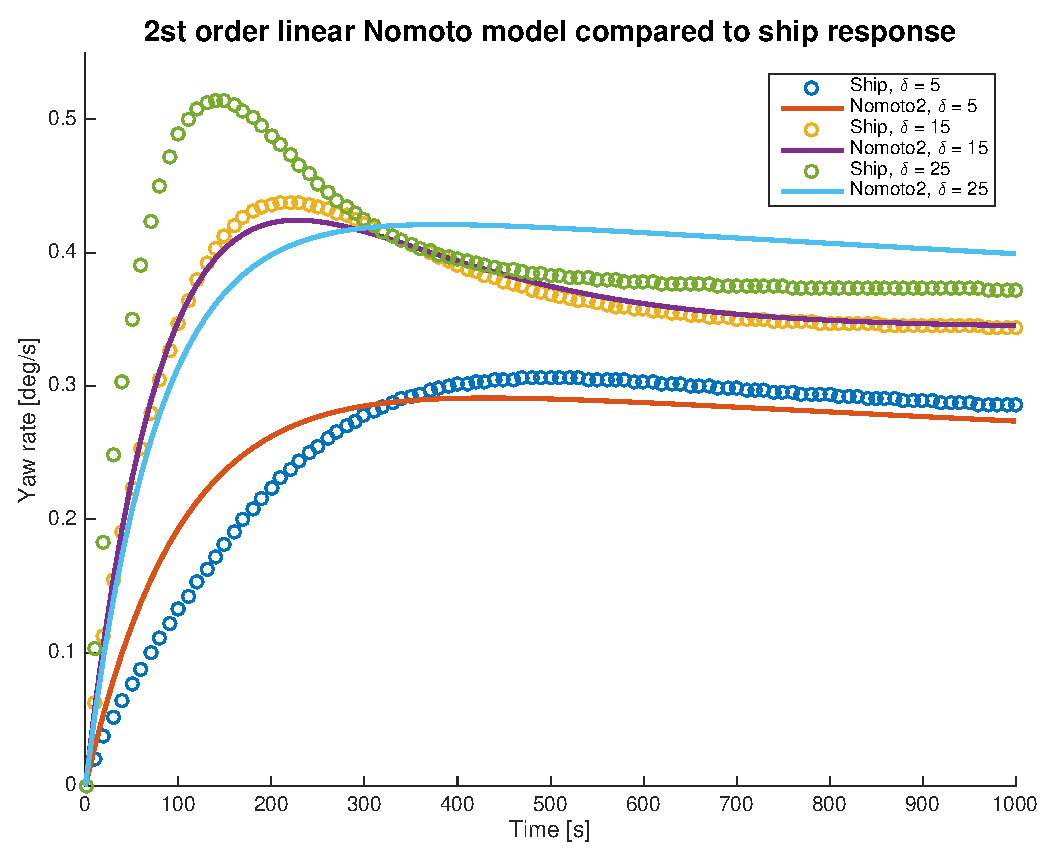
\includegraphics[width= \textwidth]{task1.4/Task1_4_Nomoto2}
    \caption{2.order linear Nomoto model}
    \label{fig:nomoto2_lin}
\end{figure}

\newpage
\subsubsection*{1. order linear Nomoto}

\begin{equation}
\begin{split}
	\frac{r}{\delta}(s) = \frac{K}{(1+Ts) } \\
	T\ddot{\psi} + \dot{\psi} = K\delta
\end{split}
\end{equation}

We also tried the first order version Nomoto, and as expected the model will only be accurate for small rudder angles, and is therefore not very good for modeling the non-linearities.

\begin{figure}[H]
    \centering
    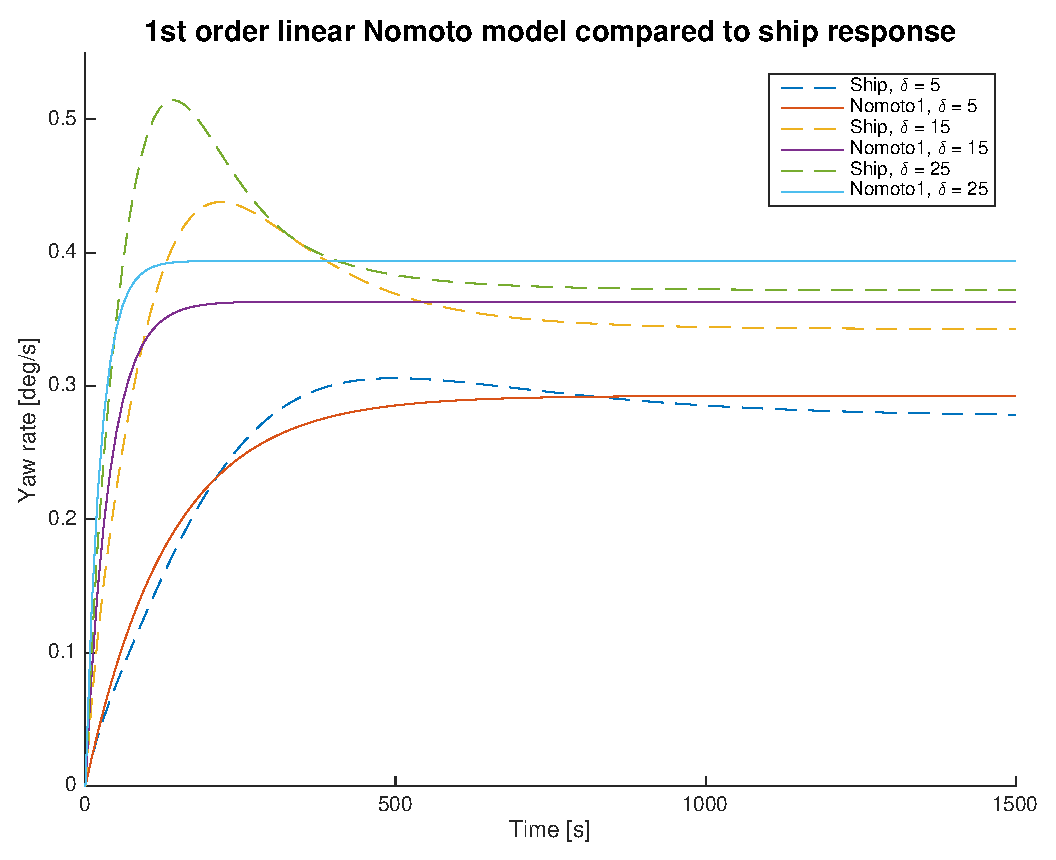
\includegraphics[width= \textwidth]{task1.4/Task1_4_Nomoto1}
    \caption{1.order linear Nomoto model}
    \label{fig:nomoto1_lin}
\end{figure}

\newpage
\subsubsection*{2. order non-linear Nomoto}
\begin{equation}
\begin{split}
	T_1 T_2 \ddot{r} + (T_1 + T_2)\dot{r} + KH_b(r) = K(\delta + T_3\dot{\delta}) \\
	H_B(r) = b_3r^3 + b_2r^2 + b_1r + b_0
\end{split}
\end{equation}
Where the steady state of $H_B(r)=\delta$. $b_0$ have already been taken care of in the fixed rudder offset, and by symmetry in the hull leads to $b_2 = 0$. We then only need the first- and third-order term to describe the maneuvering characteristics. By curve fitting $H_B(r)=b_3r^3 + b_1r=\delta$ to the obtained delta-r curve, we estimate the parameters $b_3$ and $b_1$.
\begin{figure}[H]
    \centering
    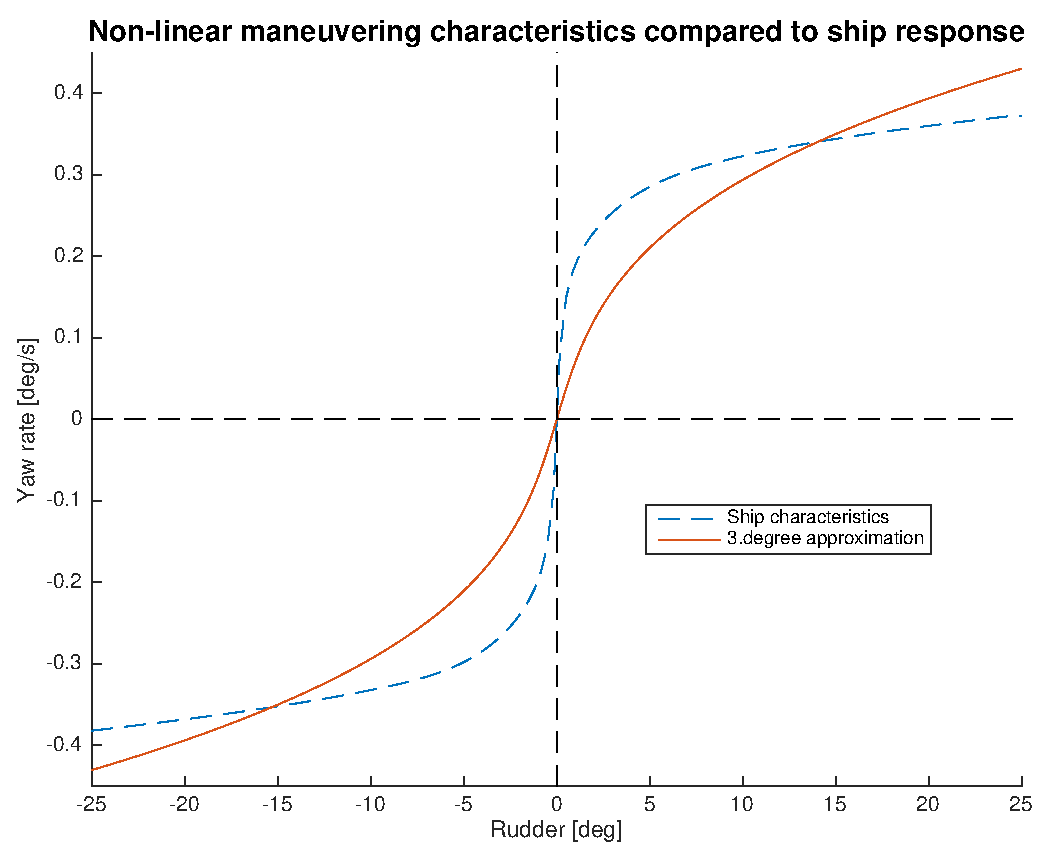
\includegraphics[width= \textwidth]{task1.4/Task1_4_Nomoto2_delta_r}
    \caption{Third degree approximation of ship characteristics}
    \label{fig:nomoto2_delta_r}
\end{figure}
    
\begin{figure}[H]
    \centering
    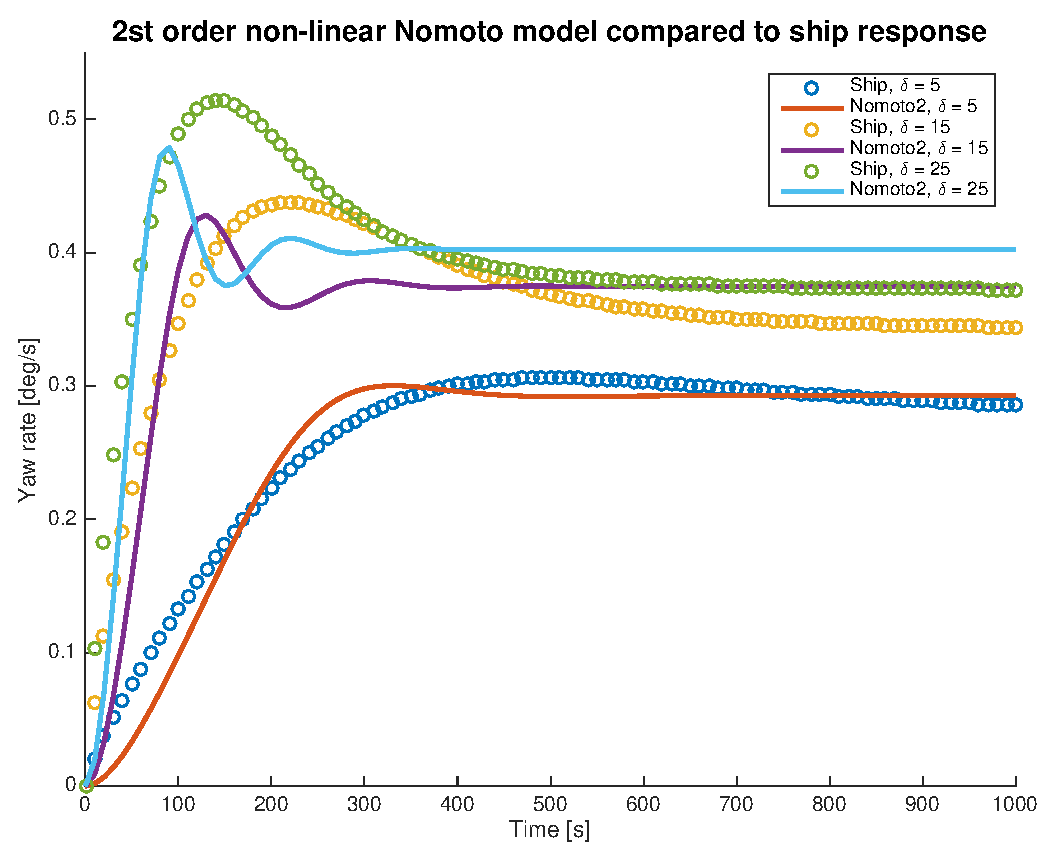
\includegraphics[width=  \textwidth]{task1.4/Task1_4_Nomoto2_curvefit}
    \caption{2.order non-linear Nomoto model}
    \label{fig:nomoto2_nonlin}
\end{figure}


\newpage
\subsubsection*{1. order non-linear Nomoto}
Norbins' extension of the linear first order model:
\begin{equation}
\begin{split}
	T\dot{r}+H_N(r)=K\delta \\
	H_N(r) = n_3r^3 + n_2r^2 + n_1r + n_0
\end{split}
\end{equation}
Where the steady state of $H_N(r)=K\delta$. We know that $n_i = \frac{b_i}{|b_1|}$, and since our ship is stable we know that $n_1=1$, and $n_3 = sign(b_3)=1$ thus resulting in following model.
\begin{equation}
\begin{split}
	T\dot{r}+r^3 + r=K\delta 
\end{split}
\end{equation}

\begin{figure}[H]
    \centering
    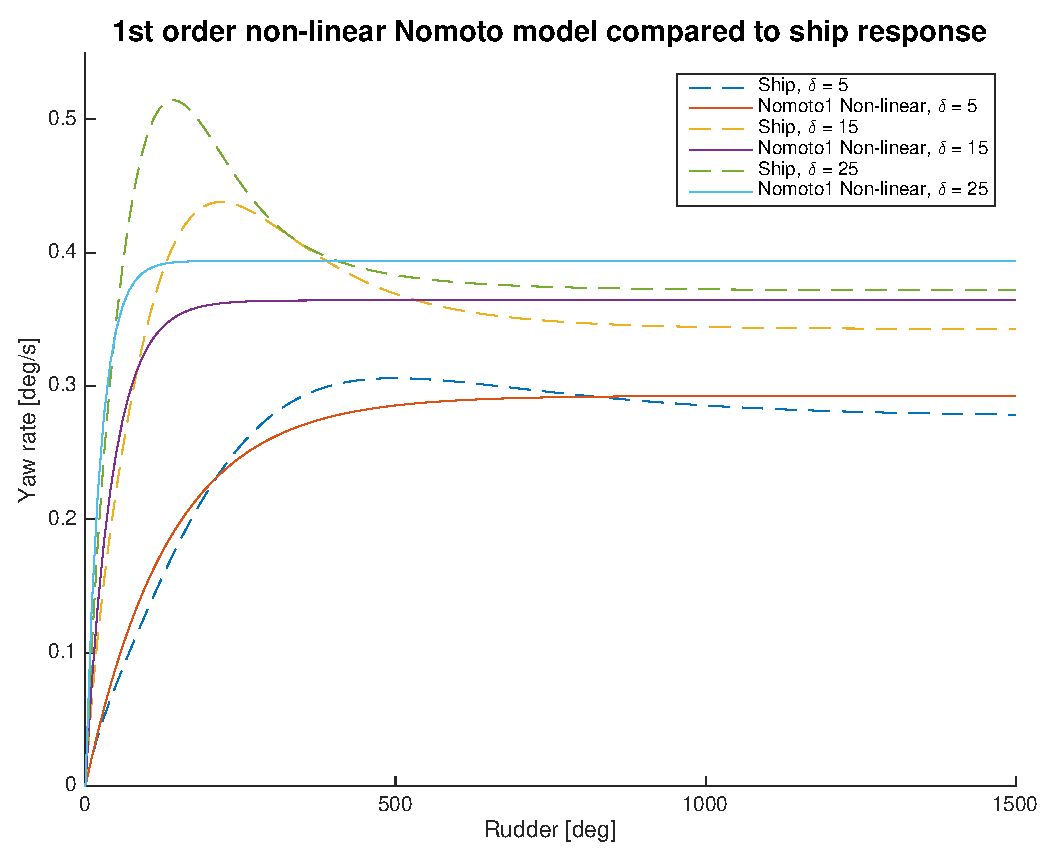
\includegraphics[width=\textwidth]{task1.4/Task1_4_Nomoto1_curvefit}
    \caption{1.order non-linear Nomoto model}
    \label{fig:nomoto1_nonlin}
\end{figure}
